
\subsection{Wersja 1}

W pierwszej wersji programu wykorzystany został tylko jeden blok wątków. Jeśli rozmiar bloku jest równy rozmiarowi macierzy to każdy z wątków oblicza 1 element wyniku. W przeciwnym przypatku każdy z wątków oblicza $$ {\left(\frac{\text{rozmiar macierzy}}{\text{rozmiar bloku}}\right)}^{2} $$ elementów wyniku. Pamięć współdzielona nie jest wykorzystywana.

\lstinputlisting[caption=Mnożenie macierzy kwadratowych na GPU -- wersja 1.]{./code/matrix_multiplication_1.cpp}

Ponieważ wykorzystany jest tylko jeden blok, obliczenia przeprowadzane są na jednym SM, a co za tym idzie w danej chwili aktywny może być tylko jeden warp. \\
Duży wpływ na prędkość przetwarzania ma wielkość bloku, dla małych bloków efektywność jest bardzo niska -- duża ilość dostępów do pamięci ogranicza prędkość przetwarzania.

\subsubsection{Czas obliczeń}

\begin{table}[H]
\centering
\begin{tabular}{|c|c|c|c|}
\hline
\multirow{2}{*}{Rozmiar macierzy} & \multicolumn{3}{c|}{Rozmiar bloku} \\ \cline{2-4}
& 8x8 & 16x16 & 22x22 \\ \hline
176x176 & 36.63 & 9.44 & 5.26 \\ \hline
352x352 & 293.13 & 74.94 & 41.96 \\ \hline
528x528 & 988.33 & 252.59 & 141.39 \\ \hline
\end{tabular}
\caption{Czas obliczeń [ms] -- wersja 1.}
\end{table}

\begin{figure}[H]
\centering
  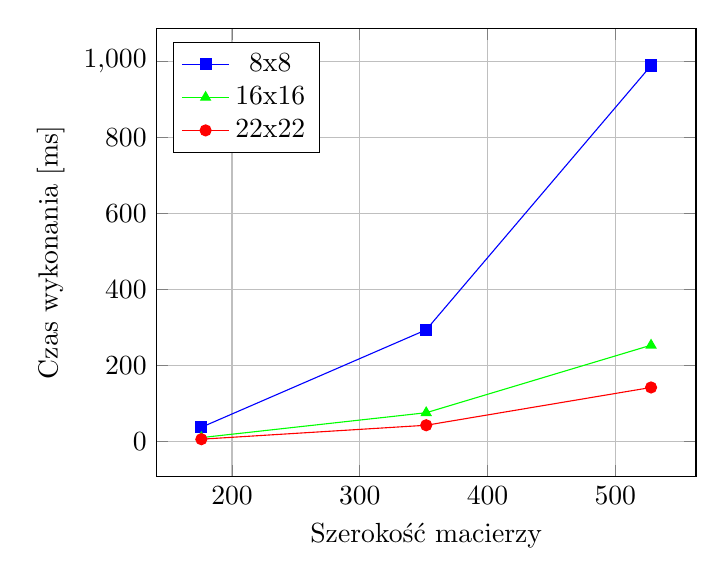
\begin{tikzpicture}
    \begin{axis}[
      xlabel=Szerokość macierzy,ylabel={Czas wykonania [ms]},legend pos= north west,grid=both]

    \addplot[color=blue,mark=square*] coordinates {
      (176, 36.63)
      (352, 293.13)
      (528, 988.33)
    };
    \addlegendentry{8x8}

    \addplot[color=green,mark=triangle*] coordinates {
      (176, 9.44)
      (352, 74.94)
      (528, 252.59)
    };
    \addlegendentry{16x16}

    \addplot[color=red,mark=*] coordinates {
      (176, 5.26)
      (352, 41.96)
      (528, 141.39)
    };
    \addlegendentry{22x22}

    \end{axis}%
  \end{tikzpicture}%
\caption{Zależność pomiędzy czasem obliczeń a rozmiarem macierzy -- wersja 1.}
\end{figure}


\subsubsection{Ilosc operacji zmiennoprzecinkowych na sekundę}

\begin{table}[H]
\centering
\begin{tabular}{|c|c|c|c|}
\hline
\multirow{2}{*}{Rozmiar macierzy} & \multicolumn{3}{c|}{Rozmiar bloku} \\ \cline{2-4}
& 8x8 & 16x16 & 22x22 \\ \hline
176x176 & 0.298 & 1.156 & 2.075 \\ \hline
352x352 & 0.298 & 1.164 & 2.079 \\ \hline
528x528 & 0.298 & 1.165 & 2.082 \\ \hline
\end{tabular}
\caption{Ilosc operacji zmiennoprzecinkowych na sekundę (GFLOPS) -- wersja 1.}
\end{table}

\begin{figure}[H]
\centering
  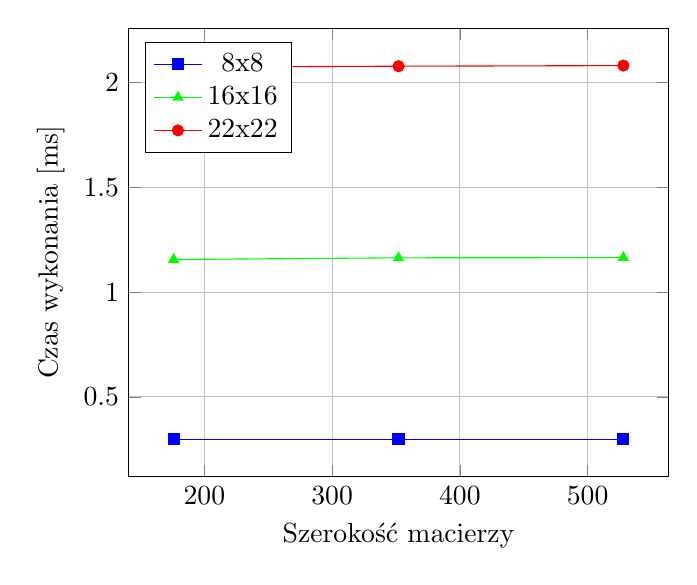
\begin{tikzpicture}
    \begin{axis}[
      xlabel=Szerokość macierzy,ylabel={Czas wykonania [ms]},legend pos= north west,grid=both]

    \addplot[color=blue,mark=square*] coordinates {
      (176, 0.298)
      (352, 0.298)
      (528, 0.298)
    };
    \addlegendentry{8x8}

    \addplot[color=green,mark=triangle*] coordinates {
      (176, 1.156)
      (352, 1.164)
      (528, 1.165)
    };
    \addlegendentry{16x16}

    \addplot[color=red,mark=*] coordinates {
      (176, 2.075)
      (352, 2.079)
      (528, 2.082)
    };
    \addlegendentry{22x22}

    \end{axis}%
  \end{tikzpicture}%
\caption{Zależność pomiędzy ilością operacji zmiennoprzecinkowychna sekundę a rozmiarem macierzy -- wersja 1.}
\end{figure}


\subsubsection{Ilość instrukcji wykonana na sekundę}

\begin{table}[H]
\centering
\begin{tabular}{|c|c|c|c|}
\hline
\multirow{2}{*}{Rozmiar macierzy} & \multicolumn{3}{c|}{Rozmiar bloku} \\ \cline{2-4}
& 8x8 & 16x16 & 22x22 \\ \hline
176x176 & 0.03328 & 0.12932 & 0.24590 \\ \hline
352x352 & 0.03290 & 0.12872 & 0.24324 \\ \hline
528x528 & 0.03281 & 0.12840 & 0.24268 \\ \hline
\end{tabular}
\caption{Ilość instrukcji wykonana na sekundę (GIPS) -- wersja 1.}
\end{table}

\begin{figure}[H]
\centering
  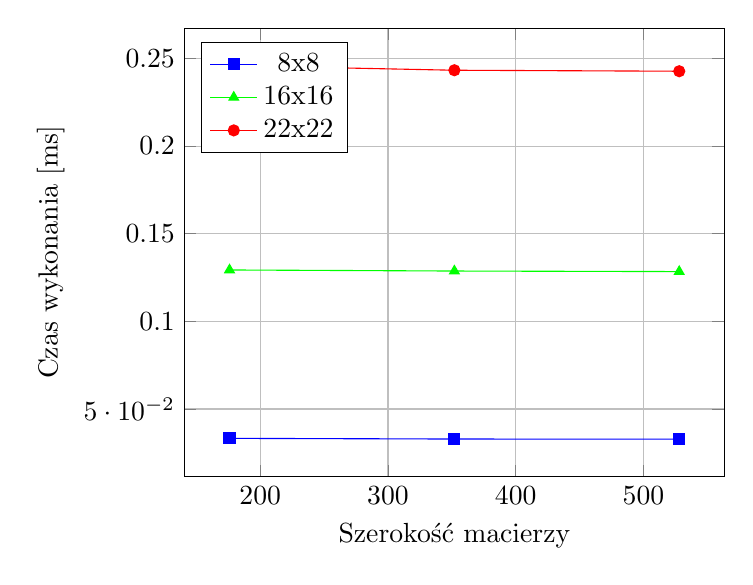
\begin{tikzpicture}
    \begin{axis}[
      xlabel=Szerokość macierzy,ylabel={Czas wykonania [ms]},legend pos= north west,grid=both]

    \addplot[color=blue,mark=square*] coordinates {
      (176, 0.03328)
      (352, 0.03290)
      (528, 0.03281)
    };
    \addlegendentry{8x8}

    \addplot[color=green,mark=triangle*] coordinates {
      (176, 0.12932)
      (352, 0.12872)
      (528, 0.12840)
    };
    \addlegendentry{16x16}

    \addplot[color=red,mark=*] coordinates {
      (176, 0.24590)
      (352, 0.24324)
      (528, 0.24268)
    };
    \addlegendentry{22x22}

    \end{axis}%
  \end{tikzpicture}%
\caption{Zależność pomiędzy ilością instrukcji wykonanych na sekundę a rozmiarem macierzy -- wersja 1.}
\end{figure}

\subsubsection{CGMA}

\begin{table}[H]
\centering
\begin{tabular}{|c|c|c|c|}
\hline
\multirow{2}{*}{Rozmiar macierzy} & \multicolumn{3}{c|}{Rozmiar bloku} \\ \cline{2-4}
& 8x8 & 16x16 & 22x22 \\ \hline
176x176 & 0.03328 & 0.12932 & 0.24590 \\ \hline
352x352 & 0.03290 & 0.12872 & 0.24324 \\ \hline
528x528 & 0.03281 & 0.12840 & 0.24268 \\ \hline
\end{tabular}
\caption{Stosunek ilości operacji zmiennoprzecinkowych do ilości operacji odczytu/zapisu z pamięci globalnej -- wersja 1.}
\end{table}

\begin{figure}[H]
\centering
  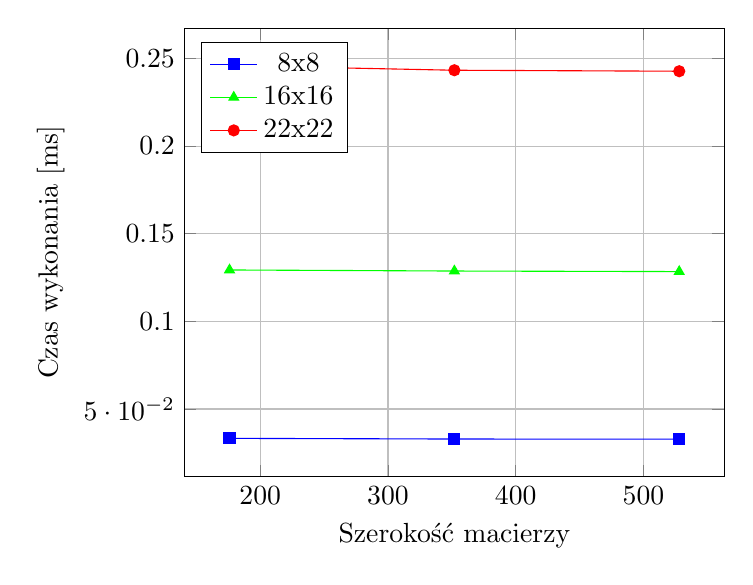
\begin{tikzpicture}
    \begin{axis}[
      xlabel=Szerokość macierzy,ylabel={Czas wykonania [ms]},legend pos= north west,grid=both]

    \addplot[color=blue,mark=square*] coordinates {
      (176, 0.03328)
      (352, 0.03290)
      (528, 0.03281)
    };
    \addlegendentry{8x8}

    \addplot[color=green,mark=triangle*] coordinates {
      (176, 0.12932)
      (352, 0.12872)
      (528, 0.12840)
    };
    \addlegendentry{16x16}

    \addplot[color=red,mark=*] coordinates {
      (176, 0.24590)
      (352, 0.24324)
      (528, 0.24268)
    };
    \addlegendentry{22x22}

    \end{axis}%
  \end{tikzpicture}%
\caption{Zależność CGMA od rozmiaru macierzy -- wersja 1.}
\end{figure}
